\documentclass{article}
\usepackage{pgfplots}

\begin{document}

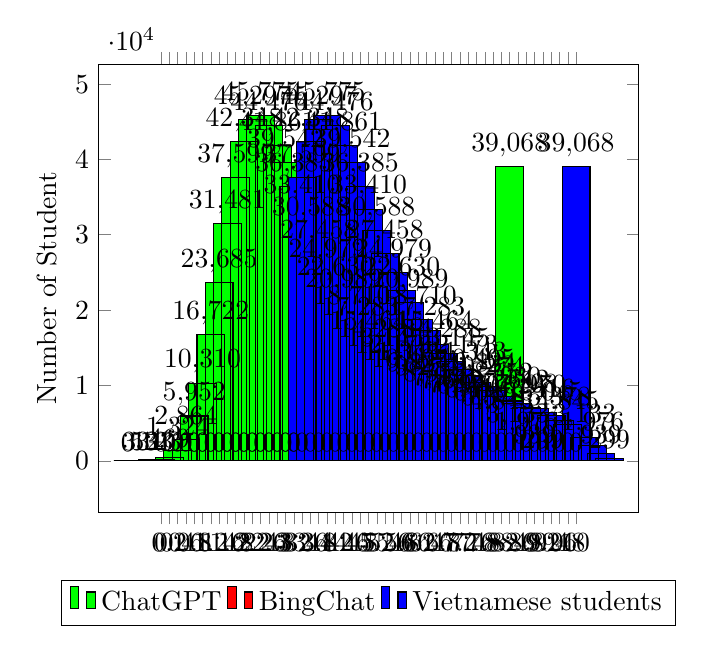
\begin{tikzpicture}
    \begin{axis}[
        ybar,
        enlargelimits=0.15,
        legend style={at={(0.5,-0.15)},
            anchor=north,legend columns=-1},
        ylabel={Number of Student},
        symbolic x coords={0, 0.2, 0.4, 0.6, 0.8, 1, 1.2, 1.4, 1.6, 1.8, 2, 2.2, 2.4, 2.6, 2.8, 3, 3.2, 3.4, 3.6, 3.8, 4, 4.2, 4.4, 4.6, 4.8, 5, 5.2, 5.4, 5.6, 5.8, 6, 6.2, 6.4, 6.6, 6.8, 7, 7.2, 7.4, 7.6, 7.8, 8, 8.2, 8.4, 8.6, 8.8, 9, 9.2, 9.4, 9.6, 9.8, 10},
        xtick=data,
        nodes near coords,
        nodes near coords align={vertical},
        ]
        \addplot[fill=green] coordinates {(0,0) (0.2,33) (0.4,53) (0.6,123) (0.8,123) (1,469) (1.2,1324) (1.4,2864) (1.6,5952) (1.8,10310) (2,16722) (2.2,23685) (2.4,31481) (2.6,37599) (2.8,42348) (3,45297) (3.2,45775) (3.4,44476) (3.6,41861) (3.8,39542) (4,36385) (4.2,33410) (4.4,30588) (4.6,27458) (4.8,24979) (5,22630) (5.2,20989) (5.4,18710) (5.6,17283) (5.8,15464) (6,14288) (6.2,13145) (6.4,12173) (6.6,11343) (6.8,10405) (7,9834) (7.2,9274) (7.4,8552) (7.6,7930) (7.8,7612) (8,7108) (8.2,6970) (8.4,6416) (8.6,6045) (8.8,5378) (9,4845) (9.2,39068) (9.4,3133) (9.6,1976) (9.8,939) (10,299)};
        \addplot[fill=red] coordinates {(0,0) (0.2,0) (0.4,0) (0.6,0) (0.8,0) (1,0) (1.2,0) (1.4,0) (1.6,0) (1.8,0) (2,0) (2.2,0) (2.4,0) (2.6,0) (2.8,0) (3,0) (3.2,0) (3.4,0) (3.6,0) (3.8,0) (4,0) (4.2,0) (4.4,0) (4.6,0) (4.8,0) (5,0) (5.2,0) (5.4,0) (5.6,0) (5.8,0) (6,0) (6.2,0) (6.4,0) (6.6,0) (6.8,0) (7,0) (7.2,0) (7.4,0) (7.6,0) (7.8,0) (8,0) (8.2,0) (8.4,0) (8.6,0) (8.8,0) (9,0) (9.2,0) (9.4,0) (9.6,0) (9.8,0) (10,0)};
        \addplot[fill=blue] coordinates {(0,0) (0.2,0) (0.4,0) (0.6,0) (0.8,0) (1,0) (1.2,0) (1.4,0) (1.6,0) (1.8,0) (2,0) (2.2,0) (2.4,0) (2.6,37599) (2.8,42348) (3,45297) (3.2,45775) (3.4,44476) (3.6,41861) (3.8,39542) (4,36385) (4.2,33410) (4.4,30588) (4.6,27458) (4.8,24979) (5,22630) (5.2,20989) (5.4,18710) (5.6,17283) (5.8,15464) (6,14288) (6.2,13145) (6.4,12173) (6.6,11343) (6.8,10405) (7,9834) (7.2,9274) (7.4,8552) (7.6,7930) (7.8,7612) (8,7108) (8.2,6970) (8.4,6416) (8.6,6045) (8.8,5378) (9,4845) (9.2,39068) (9.4,3133) (9.6,1976) (9.8,939) (10,299)};
        \legend{ChatGPT, BingChat, Vietnamese students}
    \end{axis}
\end{tikzpicture}

\end{document}